\chapter{Introduction}
% 1. Úvod

\section{About the Timepix Detectors}
%  - Historie a technické rozdíly mezi detektory typu Medipix, Medipix2, Timepix.

\section{The Timepix Network at ATLAS}
%  - Předchozí využití detektorů Medipix a software pro vizualizaci naměřených dat.
%  - Základní informace o CERN, ATLAS a síti detektorů Timepix.

\section{The Problem of Efficient Data Manipulation}
%  - Co je známo: struktura dat pro vizualizaci, jejich očekávaný objem.
%  - Co není známo: architektura systému za účelem dosažení rychlosti, robustnosti aplikace a požadovaných funkcí.
%  - Cíl práce: rozvrhnout systém, napsat serverové aplikace, definovat protokol a postavit web s vizualizací.

\section{Structure of This Document}
%  - Struktura práce.





\section{Raw Timepix Output}
%% zde je trošku Benediktovo
Timepix detectors are hybrid active pixel detectors, developed within the MPX collaboration at CERN. They consist of an active sensor layer bump-bonded to a readout ASIC. The ASIC divides the active sensor area into a square matrix of $256 \times 256$ pixels with a pixel-to-pixel distance of 55 µm. Each pixel has its own readout chain and can be controlled indenpendently. While the sensor layer material in the presented work was silicon, other sensor materials are available, most notably CdTe and GaAs, which are used e.g. for imaging applications.

Timepix detectors are operated in a way that is similar to commercially available cameras. What would be a picture in photography, is referred to as \textit{a frame}. Every pixel is equipped with a 14-bit integer register called \textit{the counter}. When acquisition starts, registers is set to zero, and then possibly incremented upon every interaction. A frame thus represents the status of each pixel after the set \textit{acqusition time}. Returning to the camera analogy, the acquisition time resembles the exposure time of a photograph---when increased, more particles are to be expected interacting with detector's pixels.

Since pixels may not be identical due to material irregularities and manufacturing errors, every pixel has adjustable \textit{threshold} parameter, which is subject to calibration. In a calibrated state, analog input measured from the pixel's semiconductor should exceed this threshold only when the pixel is interacting with a particle.

Provided that every Timepix detector installed in the ATLAS-TPX network has 2 layers of $256 \times 256$ pixel matrices, every captured frame consists of 131,072 integer values in total. Interpretation of these values depends on another parameter, \textit{the operation mode}. While it is technically possible to configure every pixel to operate in a different mode, for the desired application all pixels are set to the same mode of operation, making this essentially not a parameter of a pixel, but that of a frame. The following operation modes are available:

\begin{description}
%% CITACE: Holík 1.2.5.1 pp. 27
	\item[Hit Counting Mode (also known as the Medipix Mode)]
	In this mode, the counter is incremented upon every transition from a state below the threshold to a state above the threshold. The result is an integer value representing the number of particles which have interacted with the pixel.

	\item[Time over Threshold Mode (TOT)]\label{tpx:tot}
	In this mode, the counter is incremented by every clock cycle spent above the threshold. The result is an integer value corresponding to the energy of the interacting particle. Energy calibration methods are described in \cite{Jakubek2011S262}.

	\item[Time of Arrival Mode (TOA)]\label{tpx:toa}
	In this mode, the counter is incremented by every clock cycle after the threshold is first exceeded. The result is an integer value corresponding to the time interval before the end of the measurement.
\end{description}

\subsection{Read-out Interface}
A read-out interface is a special dedicated hardware device that reads data and controls acquisition of the detector. \cite{TurecekThesis2011} Given the harsh radiation environment within the ATLAS machine, the ATLASPIX interface was developed by modifying a regular FITPix interface.

%% CITACE: ATLASPIX at CERN

The interface has two parts connected by four cables. The detector itself is positioned and oriented within the ATLAS machine, whereas the rest of the interface is placed in a nearby server room, protected against ionizing radiation. Cables connect both parts, allowing protected hardware to control detectors remotely during operation of the machine. To manage multiple detectors simultaneously, a computer is directly connected to all read-out interfaces. This computer, also known as \textit{the control PC}, gathers all measured data and forwards commands from the system operator to the detectors through the ATLASPIX interface. This configuration is shown in Figure \ref{fig:ATLASPIX}.

At the time of writing this work, the control PC is being operated manually from a remote location. The automation of the operation is under investigation.

\begin{figure}[t]
\begin{center}
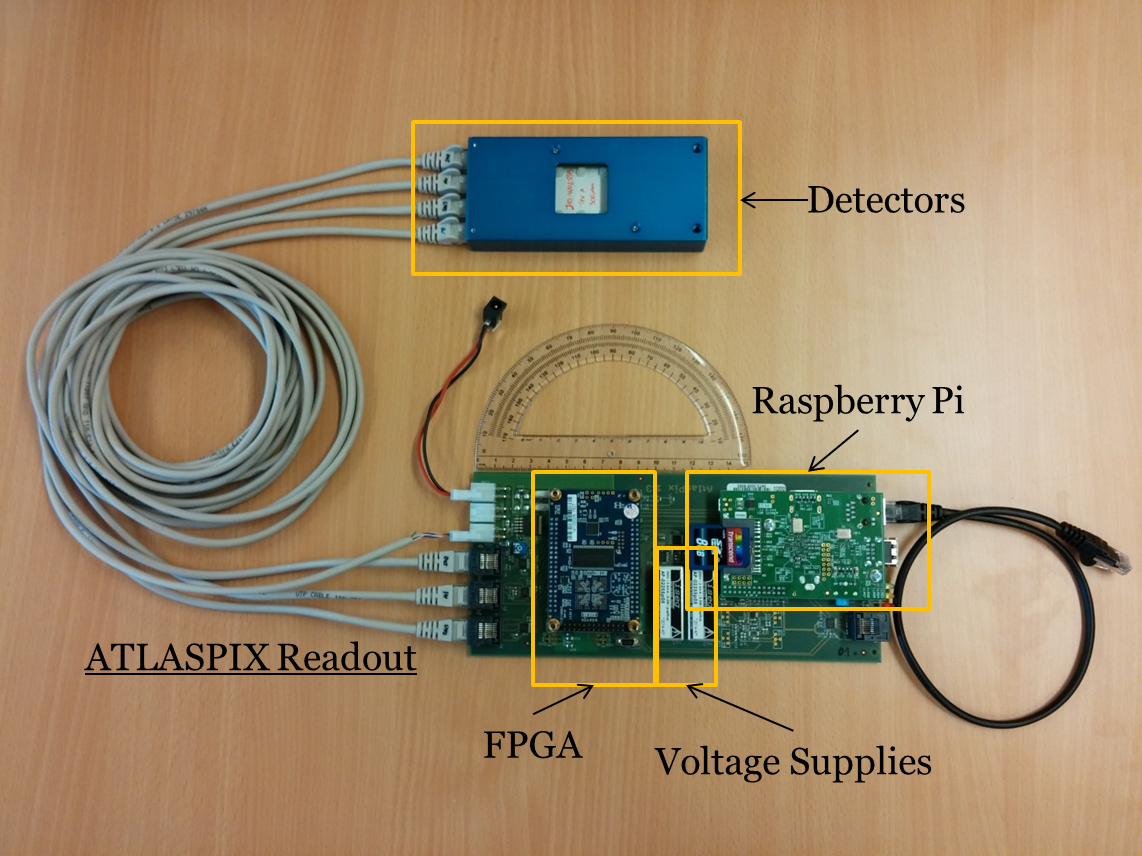
\includegraphics[height=7cm]{figures/imported/atlaspix}
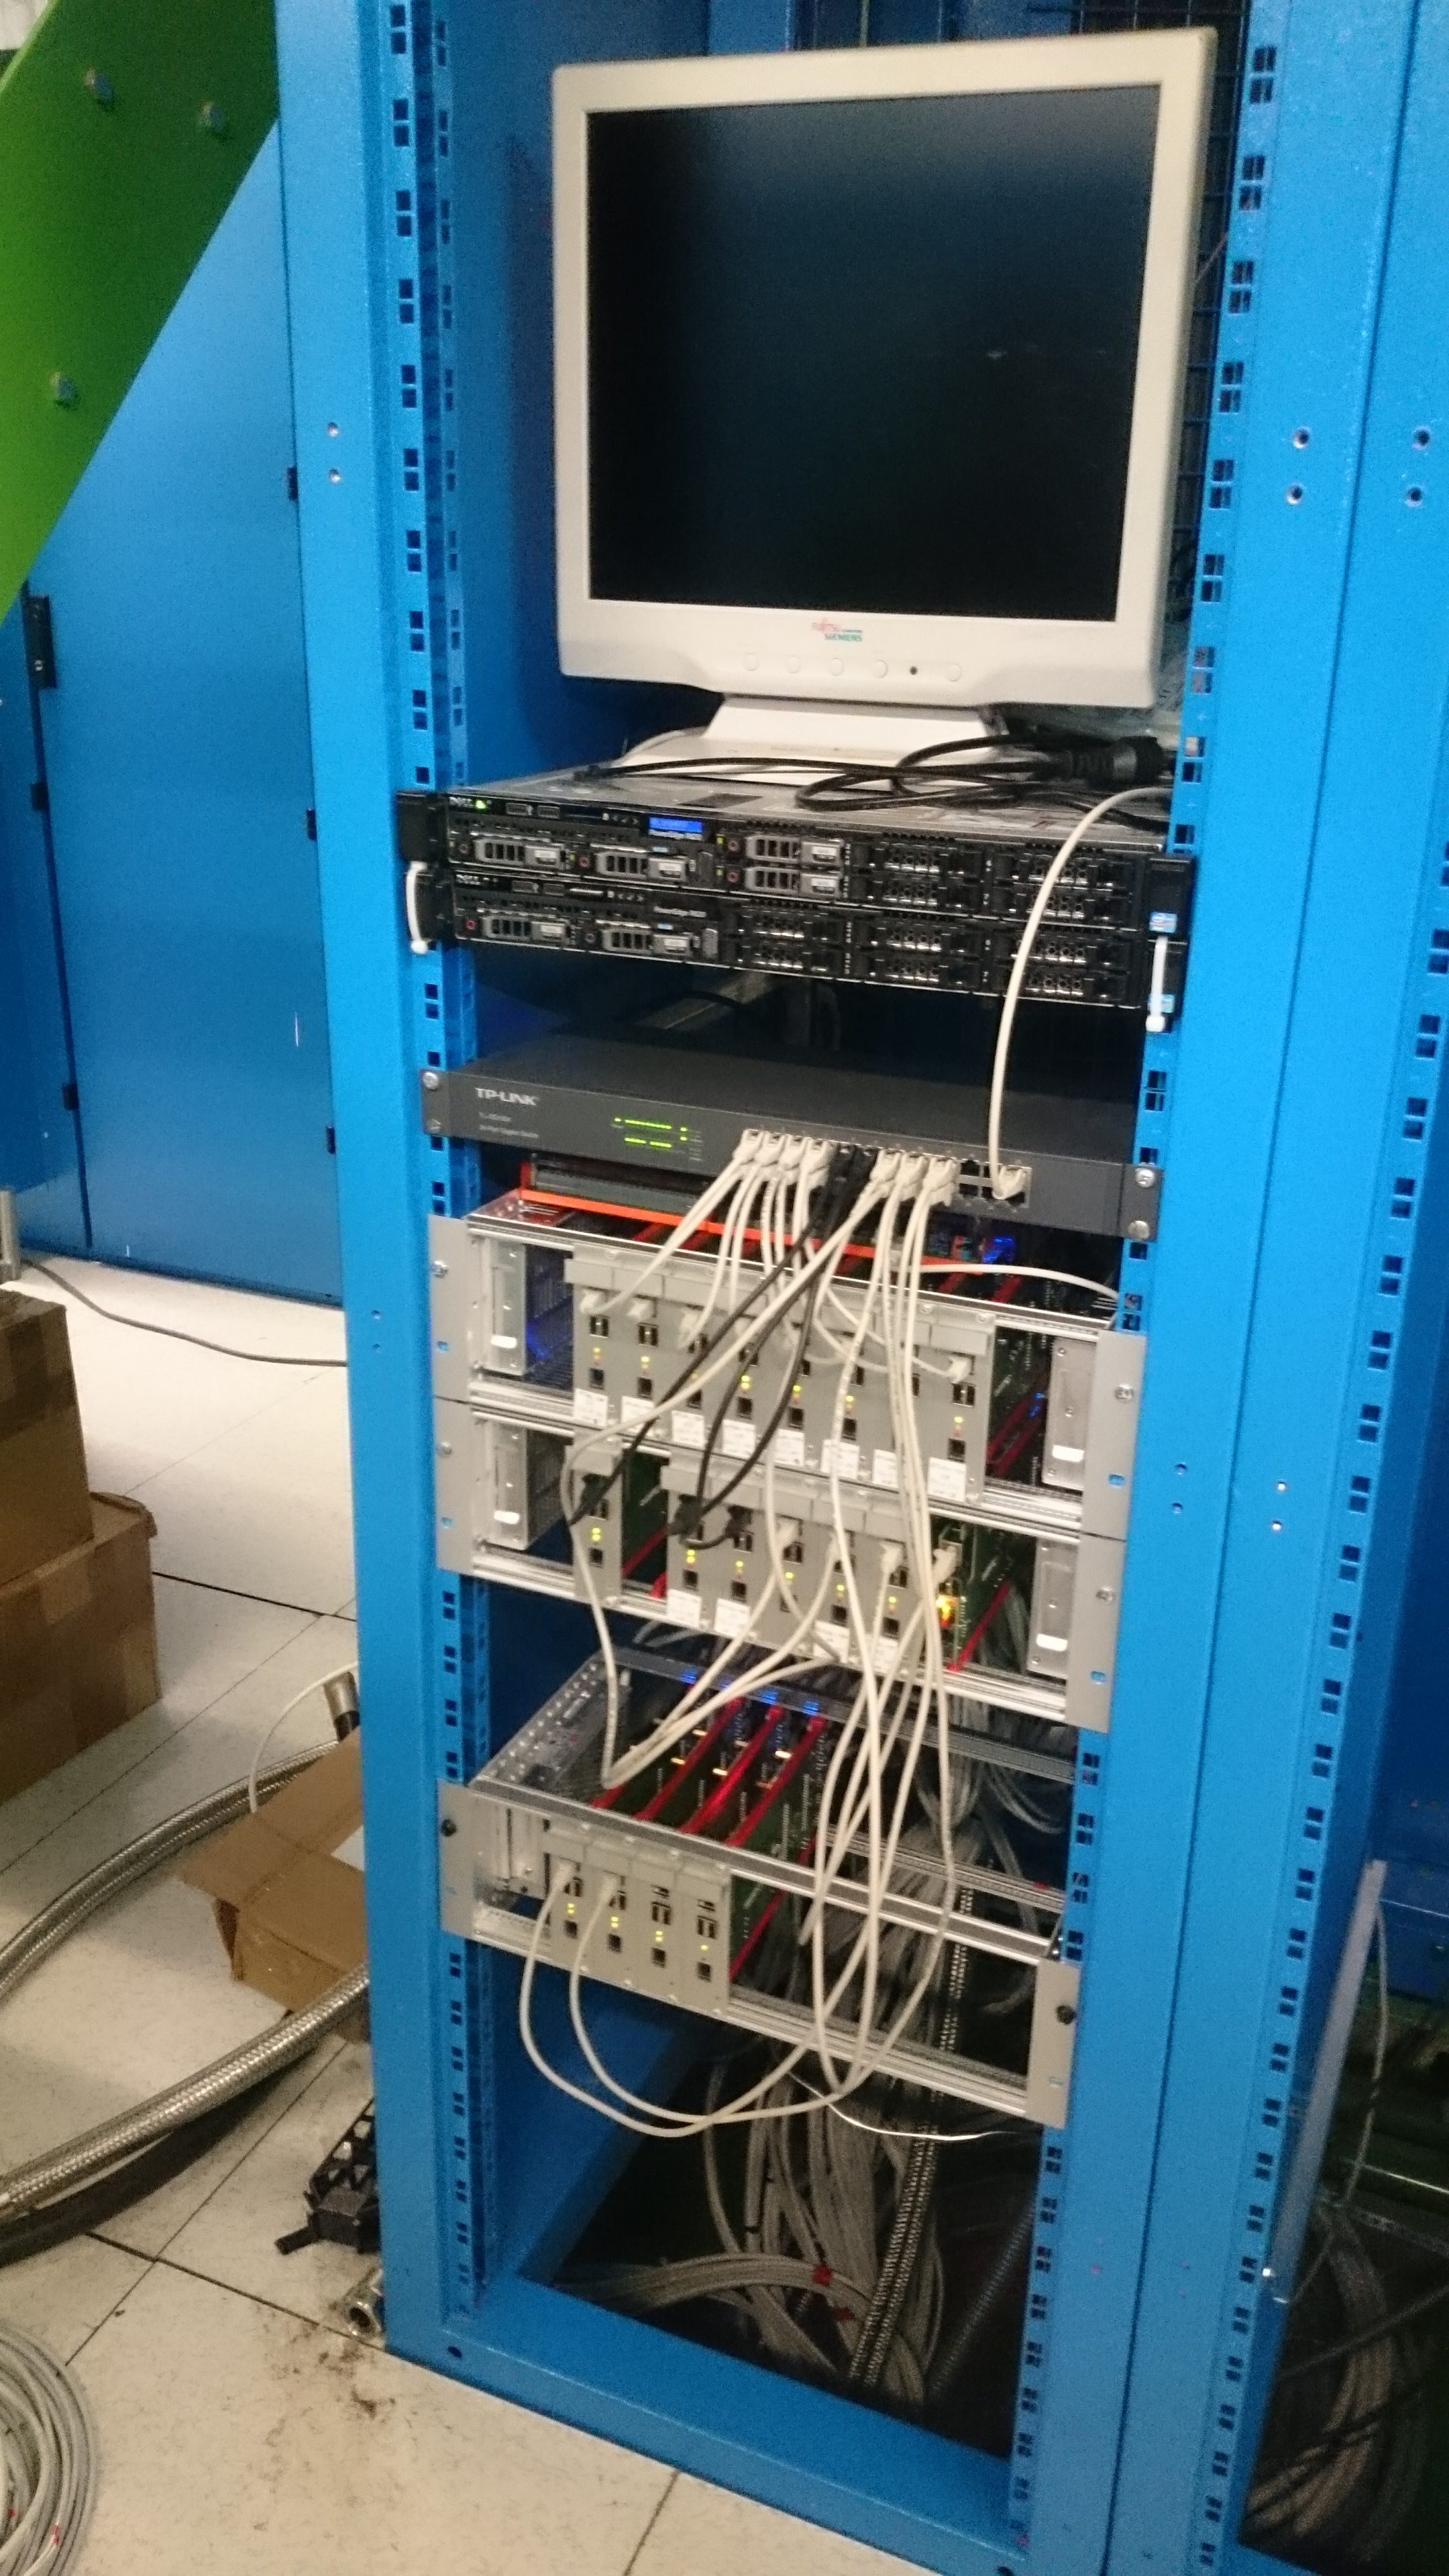
\includegraphics[height=7cm]{figures/imported/atlaspix-installed}
\caption{The ATLASPIX read-out interface installed at CERN.}
\label{fig:ATLASPIX}
\end{center}
\end{figure}

\subsection{Cluster Analysis}
%% CITACE: flood-fill
%% ZKRATKA: TOA, TOT
In ATLAS-TPX detector footage, components of various shapes and sizes can be observed, depending on the experiments performed at the time of acquisition. These components, commonly known as \textit{clusters}, are discovered and evaluated in an automated process called \textit{the cluster analysis}. This procedure involves a connectivity-checking algorithm, such as \textit{flood-fill}, operating on pixel matrices to distinguish individual clusters. In later stages, clusters are processed, measured and classified in various categories with regards to their shape. In addition, if the frame has been captured in TOT mode and calibration data are available, the automated processing script can convert counter values to energy approximations.

%% OBR: saturovaný snímek - špatně (TPX01@1441600713.82345, 2015_09_07_TPX01.root, frame #16512)
%% OBR: snímek s clustery - dobře (TPX01@1435930709.35062, 2015_07_03_TPX01.root, frame #34979)

% CITACE: sparse matrix
The output of cluster analysis consists of two separate lists of clusters, one per every sensor layer. It follows from the definition of a cluster that any pixel contained in it has a non-zero counter value. Consequently, all pixels unreferenced by any cluster are assumed to be equal to zero. The utilized technique of data encoding is well-known as it offers efficient compression rate for sparse pixel matrices. It is however worth noting at this point that in certain cases (represented most notably by saturated or nearly saturated frames), this approach produces voluminous data structures, which may take long time to enumerate, and in turn slow down other algorithms operating on them.

In a cluster list, pixels are stored as tuples of their Carthessian coordinates and their respective counter values. From this information, the pixel matrix can be reconstructed at any time. The original pixel matrix is therefore discarded without data lost at the end of the cluster analysis, in order to minimize occupied space. For every cluster, several properties are calculated in the automated processing, most notable of which are:

\label{db:cluster-properties}
\begin{description}
	\item[Shape Classification]
	\label{db:shape-classification}
	By measuring geometric properties of a cluster (such as radius or size), it is possible to estimate whether the cluster resembles more a line segment or a circular blob. Similarly, an algorithm can ascertain if the cluster looks thin or thick. From that information, type of interacting particle can be determined, along with direction of its movement relative to the plane of incidence. 

	TODO%To formally define cluster categories, we use terminology consistent with the ATLAS Medipix research (see Figure \ref{fig:cluster-types}).

    %% CITACE: Medipix cluster types

    \begin{figure}[t]
    \begin{center}

    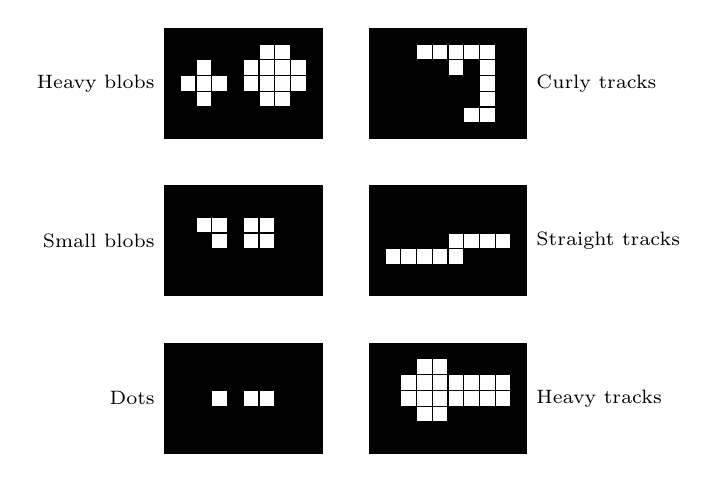
\begin{tikzpicture}
        % Dots
        \draw [fill=black] (0,0) rectangle (2,1.4);
        \draw [fill=white] (0.6,0.6) rectangle (0.8,0.8);
        \draw [fill=white] (1.0,0.6) rectangle (1.2,0.8);
        \draw [fill=white] (1.2,0.6) rectangle (1.4,0.8);
        \node[black,font=\scriptsize,anchor=east] at (0,0.7) {Dots};

        % Small blobs
        \draw [fill=black] (0,2) rectangle (2,3.4);
        \draw [fill=white] (0.6,2.6) rectangle (0.8,2.8);
        \draw [fill=white] (0.4,2.8) rectangle (0.6,3.0);
        \draw [fill=white] (0.6,2.8) rectangle (0.8,3.0);

        \draw [fill=white] (1.0,2.6) rectangle (1.2,2.8);
        \draw [fill=white] (1.2,2.6) rectangle (1.4,2.8);
        \draw [fill=white] (1.0,2.8) rectangle (1.2,3.0);
        \draw [fill=white] (1.2,2.8) rectangle (1.4,3.0);
        \node[black,font=\scriptsize,anchor=east] at (0,2.7) {Small blobs};

        % Heavy blobs
        \draw [fill=black] (0,4) rectangle (2,5.4);
        \draw [fill=white] (0.4,4.4) rectangle (0.6,4.6);
        \draw [fill=white] (0.2,4.6) rectangle (0.4,4.8);
        \draw [fill=white] (0.4,4.6) rectangle (0.6,4.8);
        \draw [fill=white] (0.6,4.6) rectangle (0.8,4.8);
        \draw [fill=white] (0.4,4.8) rectangle (0.6,5.0);

        \draw [fill=white] (1.0,4.6) rectangle (1.2,4.8);
        \draw [fill=white] (1.0,4.8) rectangle (1.2,5.0);
        \draw [fill=white] (1.2,4.4) rectangle (1.4,4.6);
        \draw [fill=white] (1.4,4.4) rectangle (1.6,4.6);
        \draw [fill=white] (1.2,4.6) rectangle (1.4,4.8);
        \draw [fill=white] (1.4,4.6) rectangle (1.6,4.8);
        \draw [fill=white] (1.2,4.8) rectangle (1.4,5.0);
        \draw [fill=white] (1.4,4.8) rectangle (1.6,5.0);
        \draw [fill=white] (1.2,5.0) rectangle (1.4,5.2);
        \draw [fill=white] (1.4,5.0) rectangle (1.6,5.2);
        \draw [fill=white] (1.6,4.6) rectangle (1.8,4.8);
        \draw [fill=white] (1.6,4.8) rectangle (1.8,5.0);
        \node[black,font=\scriptsize,anchor=east] at (0,4.7) {Heavy blobs};

        % Heavy tracks
        \draw [fill=black] (2.6,0) rectangle (4.6,1.4);
        \draw [fill=white] (3.0,0.6) rectangle (3.2,0.8);
        \draw [fill=white] (3.0,0.8) rectangle (3.2,1.0);
        \draw [fill=white] (3.2,0.4) rectangle (3.4,0.6);
        \draw [fill=white] (3.4,0.4) rectangle (3.6,0.6);
        \draw [fill=white] (3.2,0.6) rectangle (3.4,0.8);
        \draw [fill=white] (3.4,0.6) rectangle (3.6,0.8);
        \draw [fill=white] (3.2,0.8) rectangle (3.4,1.0);
        \draw [fill=white] (3.4,0.8) rectangle (3.6,1.0);
        \draw [fill=white] (3.2,1.0) rectangle (3.4,1.2);
        \draw [fill=white] (3.4,1.0) rectangle (3.6,1.2);
        \draw [fill=white] (3.6,0.6) rectangle (3.8,0.8);
        \draw [fill=white] (3.6,0.8) rectangle (3.8,1.0);
        \draw [fill=white] (3.8,0.6) rectangle (4.0,0.8);
        \draw [fill=white] (3.8,0.8) rectangle (4.0,1.0);
        \draw [fill=white] (4.0,0.6) rectangle (4.2,0.8);
        \draw [fill=white] (4.0,0.8) rectangle (4.2,1.0);
        \draw [fill=white] (4.2,0.6) rectangle (4.4,0.8);
        \draw [fill=white] (4.2,0.8) rectangle (4.4,1.0);
        \node[black,font=\scriptsize,anchor=west] at (4.6,0.7) {Heavy tracks};

        % Straight tracks
        \draw [fill=black] (2.6,2) rectangle (4.6,3.4);
        \draw [fill=white] (2.8,2.4) rectangle (3.0,2.6);
        \draw [fill=white] (3.0,2.4) rectangle (3.2,2.6);
        \draw [fill=white] (3.2,2.4) rectangle (3.4,2.6);
        \draw [fill=white] (3.4,2.4) rectangle (3.6,2.6);
        \draw [fill=white] (3.6,2.4) rectangle (3.8,2.6);
        \draw [fill=white] (3.6,2.6) rectangle (3.8,2.8);
        \draw [fill=white] (3.8,2.6) rectangle (4.0,2.8);
        \draw [fill=white] (4.0,2.6) rectangle (4.2,2.8);
        \draw [fill=white] (4.2,2.6) rectangle (4.4,2.8);
        \node[black,font=\scriptsize,anchor=west] at (4.6,2.7) {Straight tracks};

        % Curly tracks
        \draw [fill=black] (2.6,4) rectangle (4.6,5.4);
        \draw [fill=white] (3.2,5.0) rectangle (3.4,5.2);
        \draw [fill=white] (3.4,5.0) rectangle (3.6,5.2);
        \draw [fill=white] (3.6,5.0) rectangle (3.8,5.2);
        \draw [fill=white] (3.8,5.0) rectangle (4.0,5.2);
        \draw [fill=white] (4.0,5.0) rectangle (4.2,5.2);
        \draw [fill=white] (3.6,4.8) rectangle (3.8,5.0);
        \draw [fill=white] (4.0,4.8) rectangle (4.2,5.0);
        \draw [fill=white] (4.0,4.6) rectangle (4.2,4.8);
        \draw [fill=white] (4.0,4.4) rectangle (4.2,4.6);
        \draw [fill=white] (4.0,4.2) rectangle (4.2,4.4);
        \draw [fill=white] (3.8,4.2) rectangle (4.0,4.4);
        \node[black,font=\scriptsize,anchor=west] at (4.6,4.7) {Curly tracks};
    \end{tikzpicture}

    \caption{Different cluster types classified by their shapes.}
    \label{fig:cluster-types}
    \end{center}
    \end{figure}

	\item[Size, Volume]
	The size of a cluster is equal to the number of connected pixels which constitute it. The volume is a sum of counter values of those pixels.

	\item[Centroid, Volumetric Centroid]
	The centroid is defined as an unweighted average of pixel coordinates in the cluster. In analogous way, the volumetric centroid is the very same average weighted by corresponding counter values. 

	\item[Minimum and Maximum Cluster Height]
	These two figures refer to the lowest and the greatest counter values of pixels in the cluster.

	\item[Energy-based Properties \textit{(available only in TOT mode)}]
	If the energy approximations are available, many of the above-mentioned values can be also calculated with the energy substituted for counter values.
\end{description}

\section{Common Storage Formats}
\label{db:storage-formats}

\subsection{Plain Text}
%  - Multi-frame formáty, jejich výhody a nevýhody.
The most straight-forward way of storing data acquired by Timepix detectors is to use plain text files. Such output, referred to as the single-frame or the multi-frame format, commonly stores data in three files per unit of acquisition.

\begin{description}
	\item[Data File]
	Data files contain captured data from individual pixels of the detector. The data is encoded as a simple list of tuples containing pixel positions and their respective counter values. All pixels which are not mentioned are assumed to be of zero value.

	\item[Description File]
	Description files contain configuration of the detector at the time of acquisition. While there is no exhaustive definition listing every serialized parameter, description files allow to be easily extended by annotating values of parameters they store.

	To store a configuration parameter, three lines of text are required. The display name of the parameter (along with the unit or any other notes) is written on the first line. The second line describes the data type of the value and its range. The third line contains the actual value.

	\item[Index File]
	Index files contain information, which binds data files and description files together. In an index file, every frame is represented by a tuple of data addresses pointing to the first entry of the frame in the data file and the first entry in the description file.
\end{description}

Even though the plain text format has the advantage of being easily accessible with any text editor, it is disk-inefficient in terms of access speed and disk space.

\subsection{ROOT Framework}
Another storage option is the ROOT Data Analysis Framework \cite{Brun199781}. Originally concieved at CERN in 1995, the framework provides a set of powerful tools with various applications in data mining, manipulation and visualization. Unlike other similar toolkits, ROOT comes with its own machine-independent binary file format (identified by the \texttt{.root} extension). This format is designed to store enormous amounts of data within various types of data structures efficiently, while maintaining good overall performance by employing low-level memory optimization techniques and multi-tier content caching.

%% ZKRATKA: API
%% ZKRATKA: ROOT?

Used by many physicists at CERN for several years now, ROOT was chosen as the data archivation format as many researchers have already learned its caveats and know well how to operate it despite often lacking deeper background in Computer Science. For the purposes of programmatic access, ROOT also does well with documented APIs in Python, R and C++.

Should data be stored in ROOT, a basic relational database concept comes to mind. ROOT however offers even more abstract data structures with standard tables generalized in the form of \textit{trees} and their columns in the form of \textit{leaves}. One such tree would suffice for information about captured frames (such as acquisition time, operation mode, etc.) and other for a list of clusters for every frame. This schema (showcased in Figure \ref{fig:root-trees}) would efficiently abstract the entire storage structure, allowing for multiple frames to be stored in a single file, grouped for instance by a common time interval, similarly to the text file format.

\begin{figure}[t]
\begin{center}

\begin{tikzpicture}[
    every node/.style={
        draw=black,
        thick,
        anchor=west,
        inner sep=2pt,
        minimum size=1pt,
    },
    grow via three points={
        one child at (0.8,-0.7) and two children at (0.8,-0.7) and (0.8,-1.4)
    },
    edge from parent path={
        ($(\tikzparentnode\tikzparentanchor)+(.4cm,0pt)$) |- (\tikzchildnode\tikzchildanchor)
    },
    growth parent anchor=west,
    parent anchor=south west
  ]
  \node {\texttt{data.root}}
    child { node {\texttt{calibData}} 
    	child { node [draw=none] { Calibration constants } }
    	child { node [draw=none] { Detector position \& orientation } }
    }
    child [missing] {}
    child [missing] {}
    child { node {\texttt{dscData}} 
    	child { node [draw=none] { Frame 1 detector configuration } }
    	child { node [draw=none] { Frame 2 detector configuration } }
    	child { node [draw=none] { \ldots } }
    }
    child [missing] {}
    child [missing] {}
    child [missing] {}
    child { node {\texttt{clusterFile}}
    	child { node [draw=none] { Frame 1 cluster list } }
    	child { node [draw=none] { Frame 2 cluster list } }
    	child { node [draw=none] { \ldots } }
    };
\end{tikzpicture}

\caption{Structure of a ROOT file containing Timepix footage.}
\label{fig:root-trees}
\end{center}
\end{figure}

In spite of being over 20 years in development, ROOT is not perfect. Using memory monitoring tools such as \cite{nethercote2007valgrind}, we have confirmed that the C++ implementation of the ROOT framework is riddled with various memory leaks, making it unsuitable for time-extensive operations. Some might also argue, that a full tree data structure might be overly-complicated and too generalized for a simple output described in previous sections. Lastly, ROOT framework has quite a complex object structure, making it hard to learn for first-time users.

